\documentclass[12pt,fleqn]{article}\usepackage{../../common}
\begin{document}
Ders 9

Bu derste elektriksel potansiyeli biraz daha isleyecegiz, sonra potansiyel farki
elektrik alanina ilintilendirecegiz, ve son olarak potansiyel farkin 'yol
bagimsizligindan' bahsedecegiz.

Basit ornekle baslayalim, elimde bir kapasitor var diyelim,

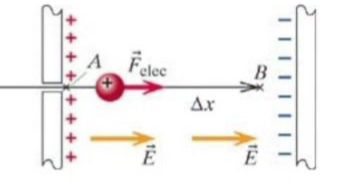
\includegraphics[width=20em]{09_01.jpg}


















\end{document}









